\title{Requirements Analysis Report}
\author{
	\textbf{Group 7} \\ \\
	Harry Stevenson \\
	Stephen Lynn \\
	David Todd \\
	Liam Joy \\
	Thomas Gak Deluen
}

\documentclass[11pt, oneside, a4paper]{article}
\usepackage[table, xcdraw]{xcolor}
\usepackage{graphicx}
\bibliographystyle{plain}

\begin{document}

\clearpage
\maketitle
\thispagestyle{empty}

\newpage
\setcounter{page}{1}

\section{Abstract}
This document is for the use of the stakeholders (Deutsche Bank) and the assessor (Professor Stephen Jarvis),
along with the software developers, it will outline the requirements of the software to be developed for
these stakeholders, for discussion in a meeting on Friday 10th February.

\section{Introduction}
We have been given a largely simplified version of the FTSE 100 stock market to identify anomalous data, we
acknowlegde that in a real-life situation, the data would be much more complex. Therefore, our system should
have the ability to be adapted to identify anomalous data in multiple different situations.

The task set is to produce software to help the stakeholders identify and flag anomalous trading patterns
on the London Stock Exchange for stocks within the FTSE 100. This is to provide an 'early warning' system
to alert the bank to rapid market changes that would be too fast to spot manually. Without this, the
stakeholders would be left vulnerable and less aware to the events causing major fluctuations within the
stock market and potentially catch rogue traders, looking to exploit the market using specified, known
techniques. The identification of such events must be done in a live data environment and the software
must be capable of coping with the fast-moving nature of the dataset required, thus human intervention
should only be required if necessary.

\section{User Requirements}
\subsection{Functional Requirements}
The Software must be able to learn the characteristics of the stocks in the FTSE 100 using a machine learning
algorithm and send an alert to notify the Business Analysts of the stakeholders when one of the following
trading patterns is detected. These characteristics will be the fluctuation amount, average, minimum and maximum
values of volumes and prices of individual stocks as well as given sectors. This will then allow the user to obtain
the relevant data to perform the root cause analysis, through the display of graphs or other relevant data display
methods. These patterns can be categorised as follows:
\begin{itemize}
	\item \textbf{Fat finger errors} -  The algorithm must be able to detect when abnormalities occur in data inputted,
	i.e. the probability of a volume or price values occurring are less than a prescribed percentage.
	\item \textbf{Pump \& Dump} - The software should check when a single or multiple trader IDs buys a large volume of
	shares and sells them shortly afterwards for the new higher price.
	\item \textbf{Bear Raid} - In a similar manner to pump \& dump, an algorithm must check that traders are not selling
	large volumes of shares to then buy them back in a short amount of time.
	\item \textbf{Volume Spikes} - This could indicate that methods such as pump \& dump or bear raids are taking place
	and thus should be monitored. The software should compare the volume of each trade to the average volume for
	this stock as determined by the machine learning algorithm which will be dependent on the fluctuation of this stock.
\end{itemize}

In doing this the software must be able to analyse both a live feed for up-to-date data, in addition to a static
csv file to analyse historical data in order to make comparisons. This historical data will also be available to
the user for them to 'drill down' into the data which caused the alert, this data should date back to the previous
two days such that meaningful short term predictions and comparisons can be made. A sample of the data that is
required to be analysed can be seen in figure \ref{SampleData}, this includes the timing of the trade, the relevant
buyer and seller, the price, volume, stock ticker symbol as well as the bid and ask prices. In this also, is the
market on which the trade was made, however this is irrelevant as this will always be the London Stock Exchange GBX.
This data should be stored in a database for it to be accessible and analysis to be performed on the data.

\begin{figure}[h]
	\label{SampleData}
	\centering
		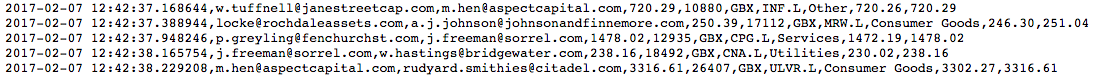
\includegraphics[width=350px]{SampleData.png}
	\caption{Data sample taken from the live data feed}
\end{figure}

The system should be able to cope with the connection and reconnection of the server from which it retrieves the
data. Therefore, when the connection resets itself at 12AM, the software should be able to disconnect safely,
retaining all data and perform the update of historical data and then be able to reconnect to the host on port 80
before 1AM when the server resumes publishing data.

The system does not require to be able to connect to any external data feeds or support multiple users, security
of the system along with the Deutsche Bank branding should not be part of the implementation.

In addition to these mandatory, primary requirements, the software may also include the following features:
Automatically organise possible trading anomalies in to the categories described above, this could then improve
the detection and tagging of anomalies in the future, through the machine learning algorithm. Cope with the
possible manipulation of whole sectors of the market or selected groups, this would allow users to browse the
data provided by market sector or by group of individual traders through a search function or tick boxes. Use
the historical data collected and archived to predict the short-term future price and volume trends, again
aiding the machine learning algorithm in deciding on thresholds beyond which trades are considered anomalous.
The user could be allowed to assist and adapt the machine learning algorithm, this will mean that it can be
tailored to a selected level of severity; however, it must be noted that the users will not be statistical or
machine learning experts so these methods for adaptation must be implemented in a simple, intuitive way.

\subsection{Non-Functional Requirements}
In addition to the functional requirements of the system, non-functional requirements describing how the system
works must also be considered for it to be effective in the workplace.

The system should always remain responsive whilst being able to process the large datasets required, thus it
should be the case that delay between a rogue trading pattern occurring and being detected and displayed is at
a minimum such that there is 5 seconds or less between the trade happening and the user being alerted to this.

The system's frontend will ensure a simple, effective display of the current system status, suggesting if action
is needed to be taken or not. This has been chosen due to the many streams of data already in possession of the
analysts utilising this software, thus it is not required to replicate all the data received, only the data of
interest for the investigation of anomalous trading patterns. This allows users of a basic understanding to
appreciate and recognise in what situations action should be taken, but also allowing the more advanced users to
access the data required to respond to such patterns successfully.

A consistent, strong user interface is important to the design of the system, similar themes should be used
throughout and the display of data should be done in an appropriate way such that it is easy to extract the
data required to understand the situation, through the use of graphs and tables for each stock as required such
that data visualisation is not excessive.

If the connection to the live data feed drops at any time during publishing of data (unless between 12am and
1am) then the system should be able to reconnect seamlessly to reduce the loss of data. The system should
therefore keep checking the connection regularly and as soon as it detects that the connection has disconnected,
then immediate reconnection should occur.

Before going live, the system will undergo rigorous testing (as laid out in the planning and design document)
to ensure its smooth running and effectiveness, this will complement such unit tests that will be made throughout
the design and implementation process.

\section{Group Management}
Through a democratic vote taken from within the group discussions, it has been decided that Thomas will take on
the role of project manager, due to his knowledge of the task in hand and the experience he has had from similar
projects in the past. He shall work alongside Stephen to create the frontend of the application, whilst still
overseeing the work of Harry, David and Liam on the frontend. The whole group will meet at least once a week in
the already discussed available timeslots between 10am and 12am on Mondays, Tuesdays, Wednesdays or Fridays, although
additional meetings may occur will necessary group members as required. All major decisions shall be taken as a group
vote, with the project manager's decision counting as final in the case of any tied votes, however, all decisions
involving the frontend or backend team only, will be taken from within the relevant team, including the project manager,
such that it allows consistency throughout the application.
The planning and design of the application will be done in the teams prescribed above, with both teams informing
each other throughout the process to ensure the feasibility and consistency of the application.

\section{Glossary}
\textbf{Fat finger errors} - human error entering data, this may include incorrectly inputting the volume
or price of trades. \\\\
\textbf{Pump \& Dump} - illegal buying of large share volumes to artificially inflate the price, by encouraging
others to follow the trend. Shares can then be sold at a higher price, yielding a large profit for the rogue trader. \\\\
\textbf{Bear Raid} - opposite to pump and dump, a trader or group of traders may short a high volume of stocks,
thus manipulating the price of the stocks, sending the price down, they will then buy back these shares at the
lower price hence making a profit. To further ensure the price of the stock will decrease, they may release false
information, detrimental to the company, thus prompting others to sell their stocks and drive the price down. \\\\
\textbf{Volume Spikes} - when compared to the average trend for the volume of trades of a share/group of shares,
if there is an unusually high volume of these stocks being traded either at once or spread out over a certain period. \\\\

\begin{thebibliography}

	\item Investopedia {\em Bear Raid} \\
	http://www.investopedia.com/terms/b/bearraid.asp \\
	Date Accessed: 07/02/2017
	\item Treanor, Jill {\em 'Fat finger trade' suspected of causing sudden FTSE fall} \\
	https://www.theguardian.com/business/2015/sep/18/fat-finger-trade-suspected-ftse-100-fall \\
	Date Accessed: 07/02/2017
	\item US Securities and Exchange Commission {\em "Pump-and-Dumps" and Market Manipulations} \\
	https://www.sec.gov/answers/pumpdump.htm \\
	Date Accessed: 07/02/2017
\end{thebibliography}

\newpage
\appendix
\section{Questions}
\textbf{Q: Should the user be able to visually see the data parsed and in what format should it be displayed?}
A: There is no specific format mandated by DB, however good data visualisation is always important when a user needs to
understand and respond to information quickly.
You should consider the use-case; traders manage portfolios containing hundreds of stocks (some of which they may not be
familiar with) and must respond quickly to events affecting any one of them. Your system needs to make a user aware something
has happened, but also furnish them with enough information to decide how to respond. I'd suggest basic information about the
stock (name, sector, price); past price, volume and volatility trend charts at minimum; and any predictions of future behaviour
your system can generate (stretch goal).  The challenge here is to provide enough information for the trader to make a purchasing
decision quickly. \\
\textbf{Q: Should we allow the user to manually adapt any characteristics learned by the machine learning algorithm?}
A: This is up to you, and is specifically mentioned as a possibility in the specification. If you do choose to allow the user
this level of control, you should be aware that the users are non-technical, meaning they are not familiar with machine learning
techniques. You should be careful to expose this functionality in a way that users can understand. \\
\textbf{Q: Is there a restriction/preferred medium of software (web app or downloadable software)?}
A: No. You are free to use any hardware or software platform at your disposal. \\
\textbf{Q: As required by the specification, our software will be able to take data from a static file. However, does this imply
that the user can at any point upload a file to the software using some means of upload implemented by us?}
A: No, not at any point. There will never be a case where a user needs to be responding to alerts from static and dynamic data
simultaneously. That said, there will be times when a user will have to upload a file to your software. \\
\textbf{Q: How long is an appropriate time frame to predict future data?}
A: This all depends on how good your predictions are. Your prediction horizon should be as long as your model is accurate for,
and no longer. It is important to note here that 'prediction' does not mean you have to specify an exact price at an exact time
in the future. It is more important to show the overall trend in the data. A model which can provide accurate projections for the
next hour or more would be considered very valuable.


\end{document}
